%% Template file for all Software/Hardware modules

\subsection{ZigBee Standard}
ZigBee is a standard that uses IEEE 802.15.4 wireless protocol as it's foundation. It's 
particularly useful for setting up ad-hoc mesh networks. Much like how any Bluetooth
devices can talk to each other, any ZigBee devices nearby can talk to each other (so 
long as they have the proper permissions).

\subsubsection{Why ZigBee?}
The advantage of using ZigBee is that it lines up with the requirements of the POW-R
project. It's a specification targeted for low-power, low-data applications that need
to be secure. 

Another advantage of using ZigBee is that XBee radios, which also fit the requirements
of the POW-R project, are ZigBee-compliant, so the forming of a mesh network can happen
quickly and easily.

\subsubsection{Device Types}
The nodes of a ZigBee network are obviously ZigBee devices, but from the network's
perspective, there are three distinct types of ZigBee devices:

\begin{itemize}
	\item Coordinator
	\item Router
	\item End Device
\end{itemize}

The coordinator runs the network, keeps it healthy, makes sure everybody is talking when
they should be, and overall, just maintains the Mesh. It is also the device that is 
typically plugged into a computer via USB or some other serial interface, meaning
that this is the node you want to send data to. There cannot be a ZigBee network
without exactly one coordinator.

Routers are fully functional ZigBee modules, capable of taking care of themselves and
routing messages across the Mesh. Routers are capable of being "parent" devices.

End devices are low-power ZigBee devices that don't do any routing. They can only talk
to one other device, which is referred to as it's "parent" device. Only a router or a coordinator
may be a parent device.

In the POW-R project, the coordinator will be attached to the Server so that it may
also act as a data bridge between the Server and the Satellites. The rest of the 
Satellites are routers; There will be no end devices in the POW-R's mesh network.


\subsubsection{Network Topology}
Zigbee supports four network topologies, shown in Figure \ref{NetTopo}. A ZigBee network
is defined by two rules:

\begin{itemize}
	\item A ZigBee network must have two or more ZigBee devices
	\item One of those devices \emph{must} be a coordinator
\end{itemize}

As mentioned before, the POW-R project will use the Mesh configuration, but without end 
devices. This means that the Mesh will consist entirely of routers and one coordinator.

\begin{figure}
\centering
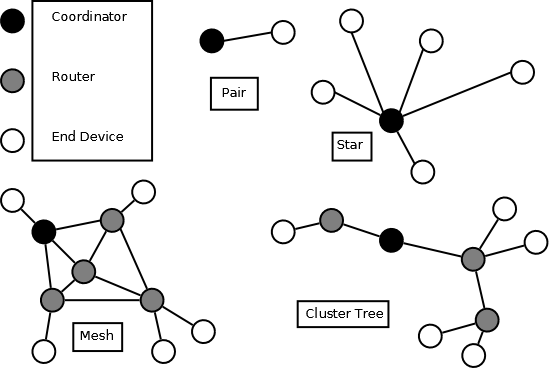
\includegraphics[scale=0.3]{Hardware/images/ZigBeeNetworkTypes.png}
\caption{ZigBee Network Topologies}
\label{NetTopo}
\end{figure}